% --------------------------------------------------------------
% This is all preamble stuff that you don't have to worry about.
% Head down to where it says "Start here"
% --------------------------------------------------------------
 
\documentclass[12pt]{article}
 
\usepackage[margin=1in]{geometry} 
\usepackage{amsmath,amsthm,amssymb}
\usepackage{graphicx}
\usepackage{epstopdf}

\newcommand{\N}{\mathbb{N}}
\newcommand{\Z}{\mathbb{Z}}
 
\newenvironment{theorem}[2][Theorem]{\begin{trivlist}
\item[\hskip \labelsep {\bfseries #1}\hskip \labelsep {\bfseries #2.}]}{\end{trivlist}}
\newenvironment{lemma}[2][Lemma]{\begin{trivlist}
\item[\hskip \labelsep {\bfseries #1}\hskip \labelsep {\bfseries #2.}]}{\end{trivlist}}
\newenvironment{exercise}[2][Exercise]{\begin{trivlist}
\item[\hskip \labelsep {\bfseries #1}\hskip \labelsep {\bfseries #2.}]}{\end{trivlist}}
\newenvironment{reflection}[2][Reflection]{\begin{trivlist}
\item[\hskip \labelsep {\bfseries #1}\hskip \labelsep {\bfseries #2.}]}{\end{trivlist}}
\newenvironment{proposition}[2][Proposition]{\begin{trivlist}
\item[\hskip \labelsep {\bfseries #1}\hskip \labelsep {\bfseries #2.}]}{\end{trivlist}}
\newenvironment{corollary}[2][Corollary]{\begin{trivlist}
\item[\hskip \labelsep {\bfseries #1}\hskip \labelsep {\bfseries #2.}]}{\end{trivlist}}
 
\begin{document}
 
% --------------------------------------------------------------
%                         Start here
% --------------------------------------------------------------
 
%\renewcommand{\qedsymbol}{\filledbox}
 
\title{Experiments of different directions in optimization for small neural networks}%replace X with the appropriate number
% \author{Chenxin} %if necessary, replace with your course title
\date{\vspace{-10ex}}
\maketitle
 

\section{The problem and the data}


I only focus on two simple networks and two sets of one dimensional data.


Network 1 (N1) has the $1-2-1$ structure, thus has 7 parameters in total. Network 2 (N2) has the $1-1-1$ structure, thus has $4$ parameters in total. I tried linear, Relu, sigmoid as three activation functions and square loss as the loss function. However, for simplicity, here all the results are based on sigmoid activation function only. Figure~\ref{fig:n} shows the network structure.
\begin{figure}[h]
\centering
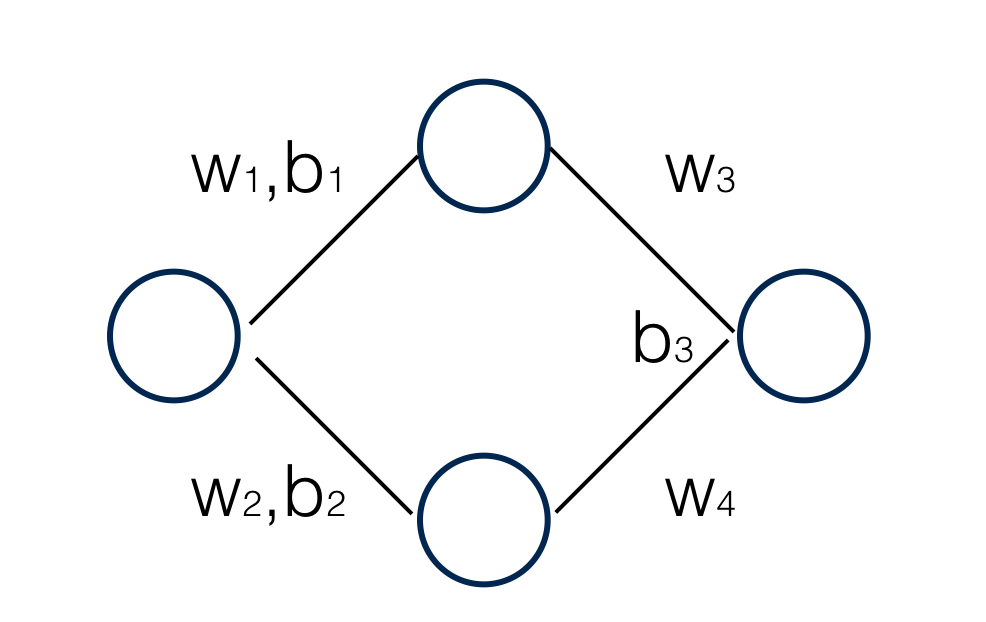
\includegraphics[width=6cm]{n1}
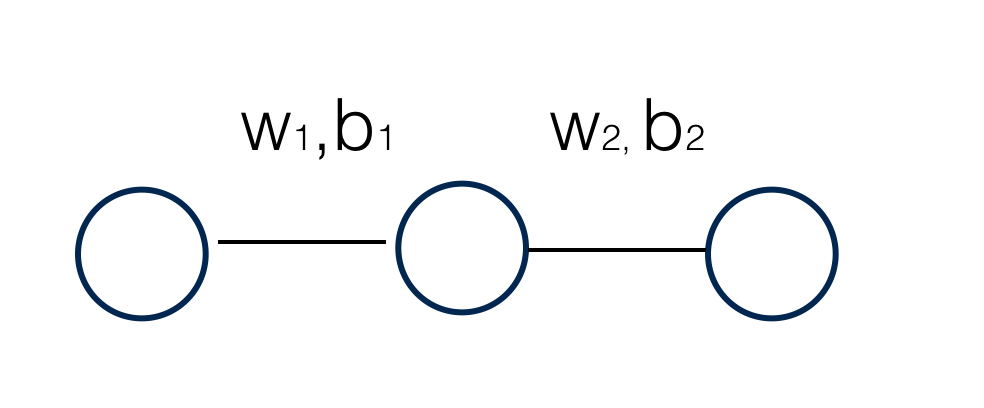
\includegraphics[width=6cm]{n2}
\caption{N1 (left) and N2 (right).}
\label{fig:n}
\end{figure}

Dataset one (D1) contains $4$ samples, two in each class. Dataset two (D2) contains $20$ samples, $10$ in each class. Figure~\ref{fig:d}  shows the distribution of both of them.
\begin{figure}[h]
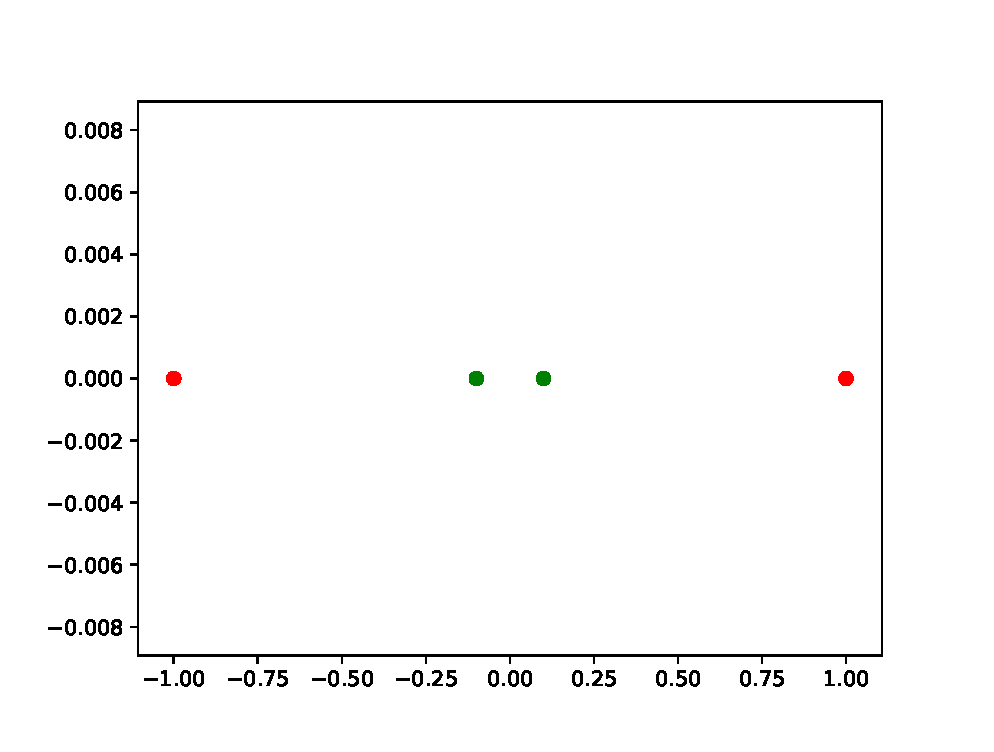
\includegraphics[width=8cm]{data1.eps}
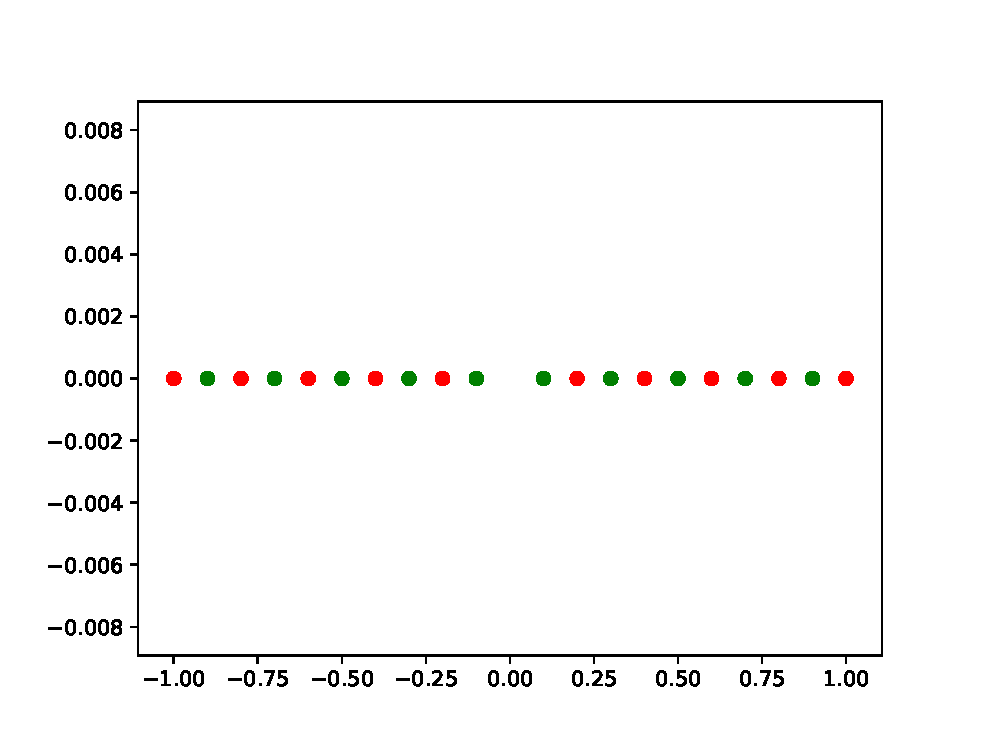
\includegraphics[width=8cm]{data2.eps}
\caption{D1 (left) and D2 (right). Red samples have $1$-label, while green samples have $0$-label.}
\label{fig:d}
\end{figure}

Notice that for D1, N1 should be able to achieve $100\%$ accuracy after training, but D2 is a rather ``difficult'' dataset for both these two networks.

\section{What directions that CG gives us?}

Here we focus on N1 only. We choose $200$ random points in ${\bf R}^7$ for initializing parameters. For each point, the gradient $d_{gd}$ and the results of CG steps $d_{cg}$ are computed. After line search, we are able to obtain two updated points and their objective values, i.e., $f_{gd}$ and $f_{cg}$. We record the ratio
$$ r:=\frac{f_{gd} - f_0}{f_{cg} - f_0 } $$
to measure the ``quality'' of two updates, where $f_0$ is the original objective value before taking any updates. Thus, $r>1$ means negative gradient could lead to more decreasing on objective value than a CG step, and vice versa.

The only difference between CG implemented here and traditional CG is, here if $\alpha<0$, we will terminate CG loops and return the negative curvature direction as output. 

The number of maximal CG iterations is tuned from $1$ to $5$.

We apply backtrack line search in both gradient steps and CG steps. The initial step size is $10$ and multiplier on it is $0.5$ if the iteration has to go on. However, for CG steps, we need to flip the sign of step size in each line search iterations since the direction may not be a descent direction. 
 
\begin{figure}[h]
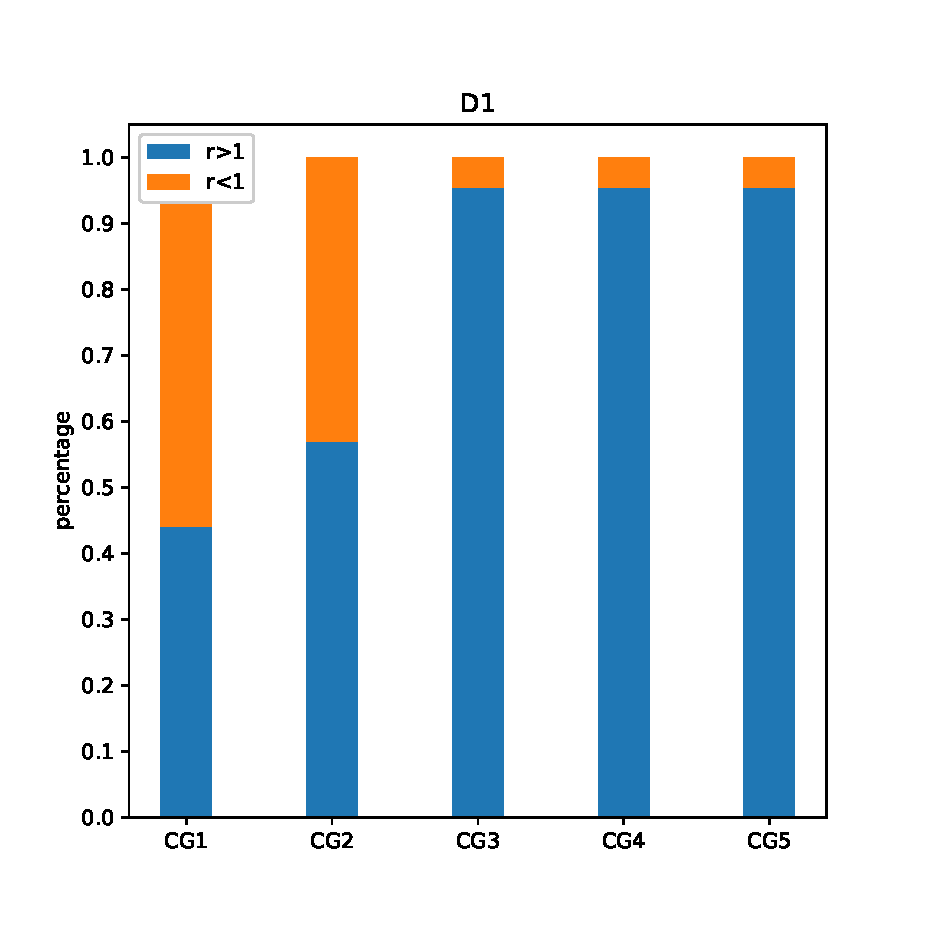
\includegraphics[width=8cm]{CGD1.eps}
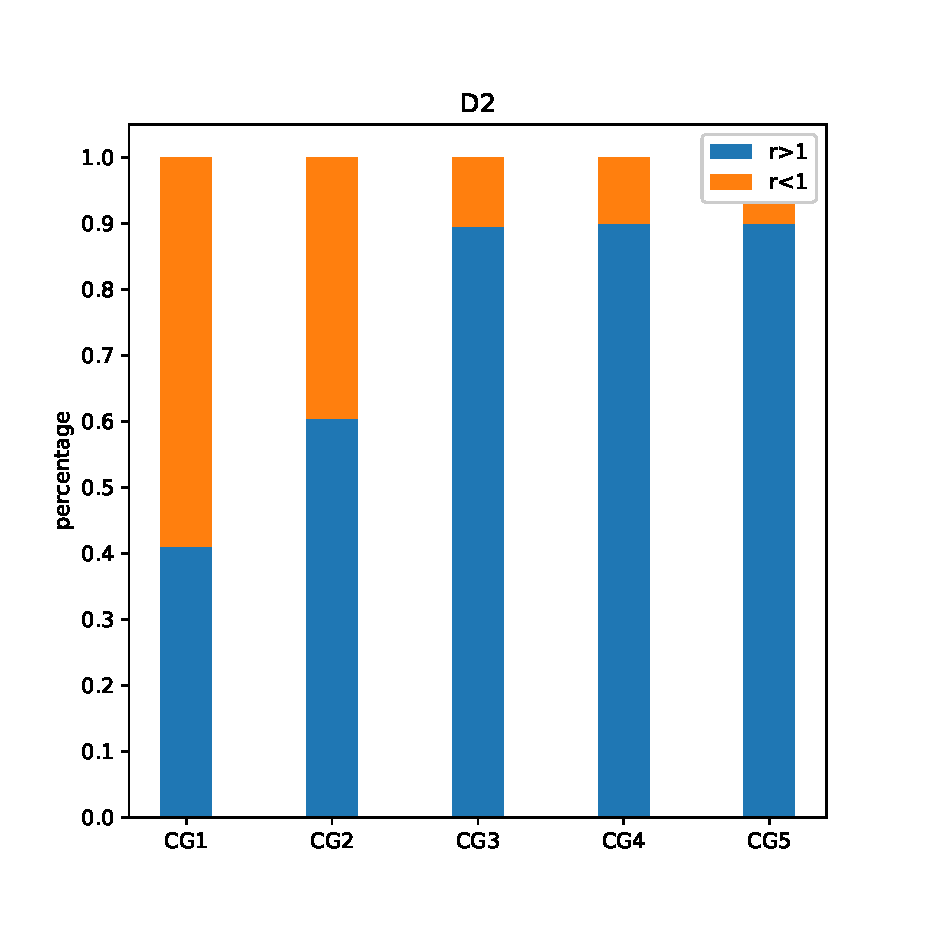
\includegraphics[width=8cm]{CGD2.eps}
\caption{Comparing negative gradient directions and CG outputs as search directions for D1 (left) and D2 (right). $r>1$ means negative gradient directions provides larger decrease on objective.}
\label{fig:CGvsGD}
\end{figure}

The figures above are two bar plots showing, by setting different maximal iterations for CG, the percentages of $r>1$ and $r<1$. The observation is that, running more than $3$ iterations of CG does not change the results at all. The reason is that CG will find a negative curvature direction in first $3$ iterations in all cases. 

Another observation is, by allowing CG to take more iterations, the outputs of CG have lower chance to beat gradient direction. Therefore, I guess the reason here is those negative curvature directions cannot provide much decrease on objective.


\section{How is leftmost eigenvector of Hessian?}

Here we consider to use leftmost eigenvector as the direction to make updates. In particular, at any point, if the leftmost eigenvalue of Hessian is less than $0$, then we use left most eigenvector to do line search. If it is greater than $0$, then we use the output of CG with $5$ as maximal number of iterations. (It is worthwhile to note that for N1 and both datasets, as far as I see, all the random points have negative leftmost eigenvalue in the Hessian.)

Let $f_{le}$ denote the objective obtained from doing line search on leftmost eigenvector as a direction. After defining
$$ r:=\frac{f_{gd} - f_0}{f_{nc} - f_0 }.$$
and running the experiments, I found there are $\mathbf{26\%}$ cases which lead to $r>1$ for D1 and $\mathbf{19\%}$ cases leading to $r>1$ for D2. The results indicate that leftmost eigenvector of Hessian could be a direction that has larger chance to lead to a larger decrease in objective than gradient. This also suggest that the negative curvature directions returned by CG is not ``negative enough'' since the product $p^TA p$ (even though it is negative) can be rather close to $0$.

\begin{figure}[h]
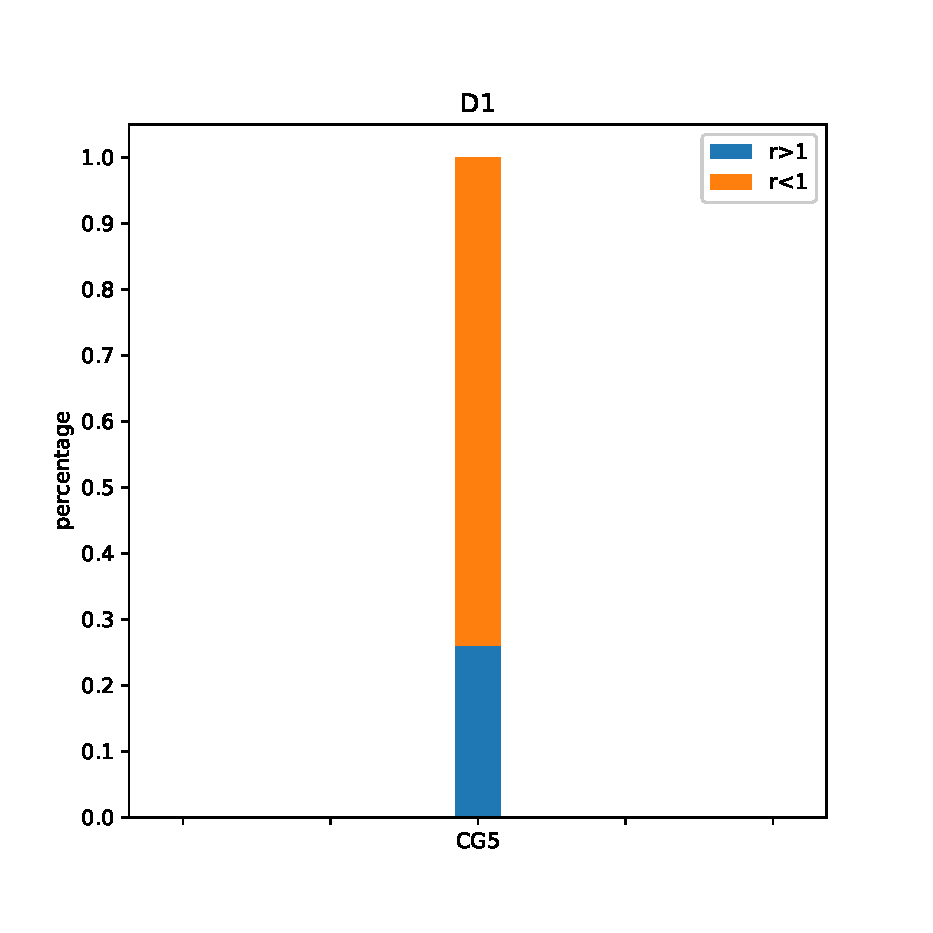
\includegraphics[width=8cm]{ncd1.eps}
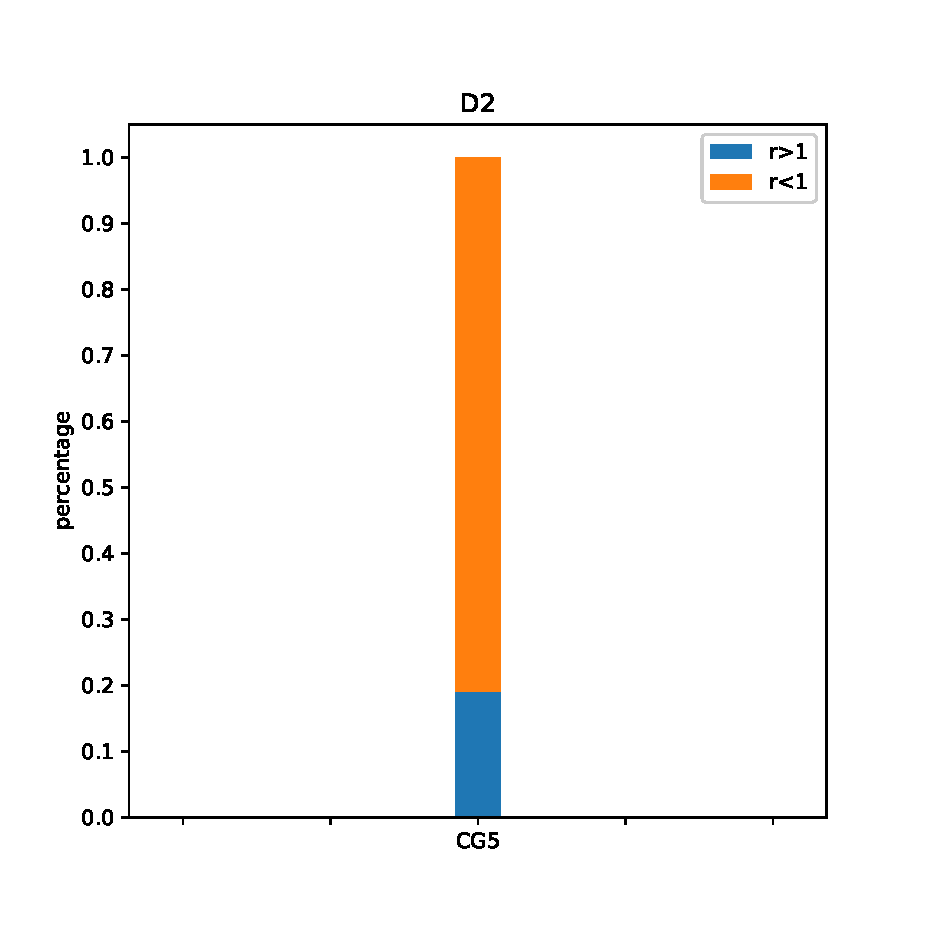
\includegraphics[width=8cm]{ncd2.eps}
\caption{Comparing negative gradient directions and leftmost eigenvectors as search directions for D1 (left) and D2 (right).  $r>1$ means negative gradient directions provides larger decrease on objective.}
\label{fig:CGvsGD}
\end{figure}


\section{Using three directions as three algorithms for training.}

In the above experiments, we compare reduction of three kinds of directions on random initial points. Here, we run each of them as an algorithm to see how they will perform on N1 and D1. In particular, each algorithm is run for $100$ iterations to see what is result it can reach.


Figure~\ref{fig:3m} is a screenshot of running each algorithms for $100$ iterations, starting with $10$ different initial points as $10$ sets of experiments. The observation is that CG can reach loss close to $0$ in most of cases, while the other two cannot. This is opposite to the observation in the previous experiments which show CG steps have lower chance to provide large decreases on objective, compared with graident steps. This is a surprising result, and I would like to explore the reason behind it.



\begin{figure}[h]
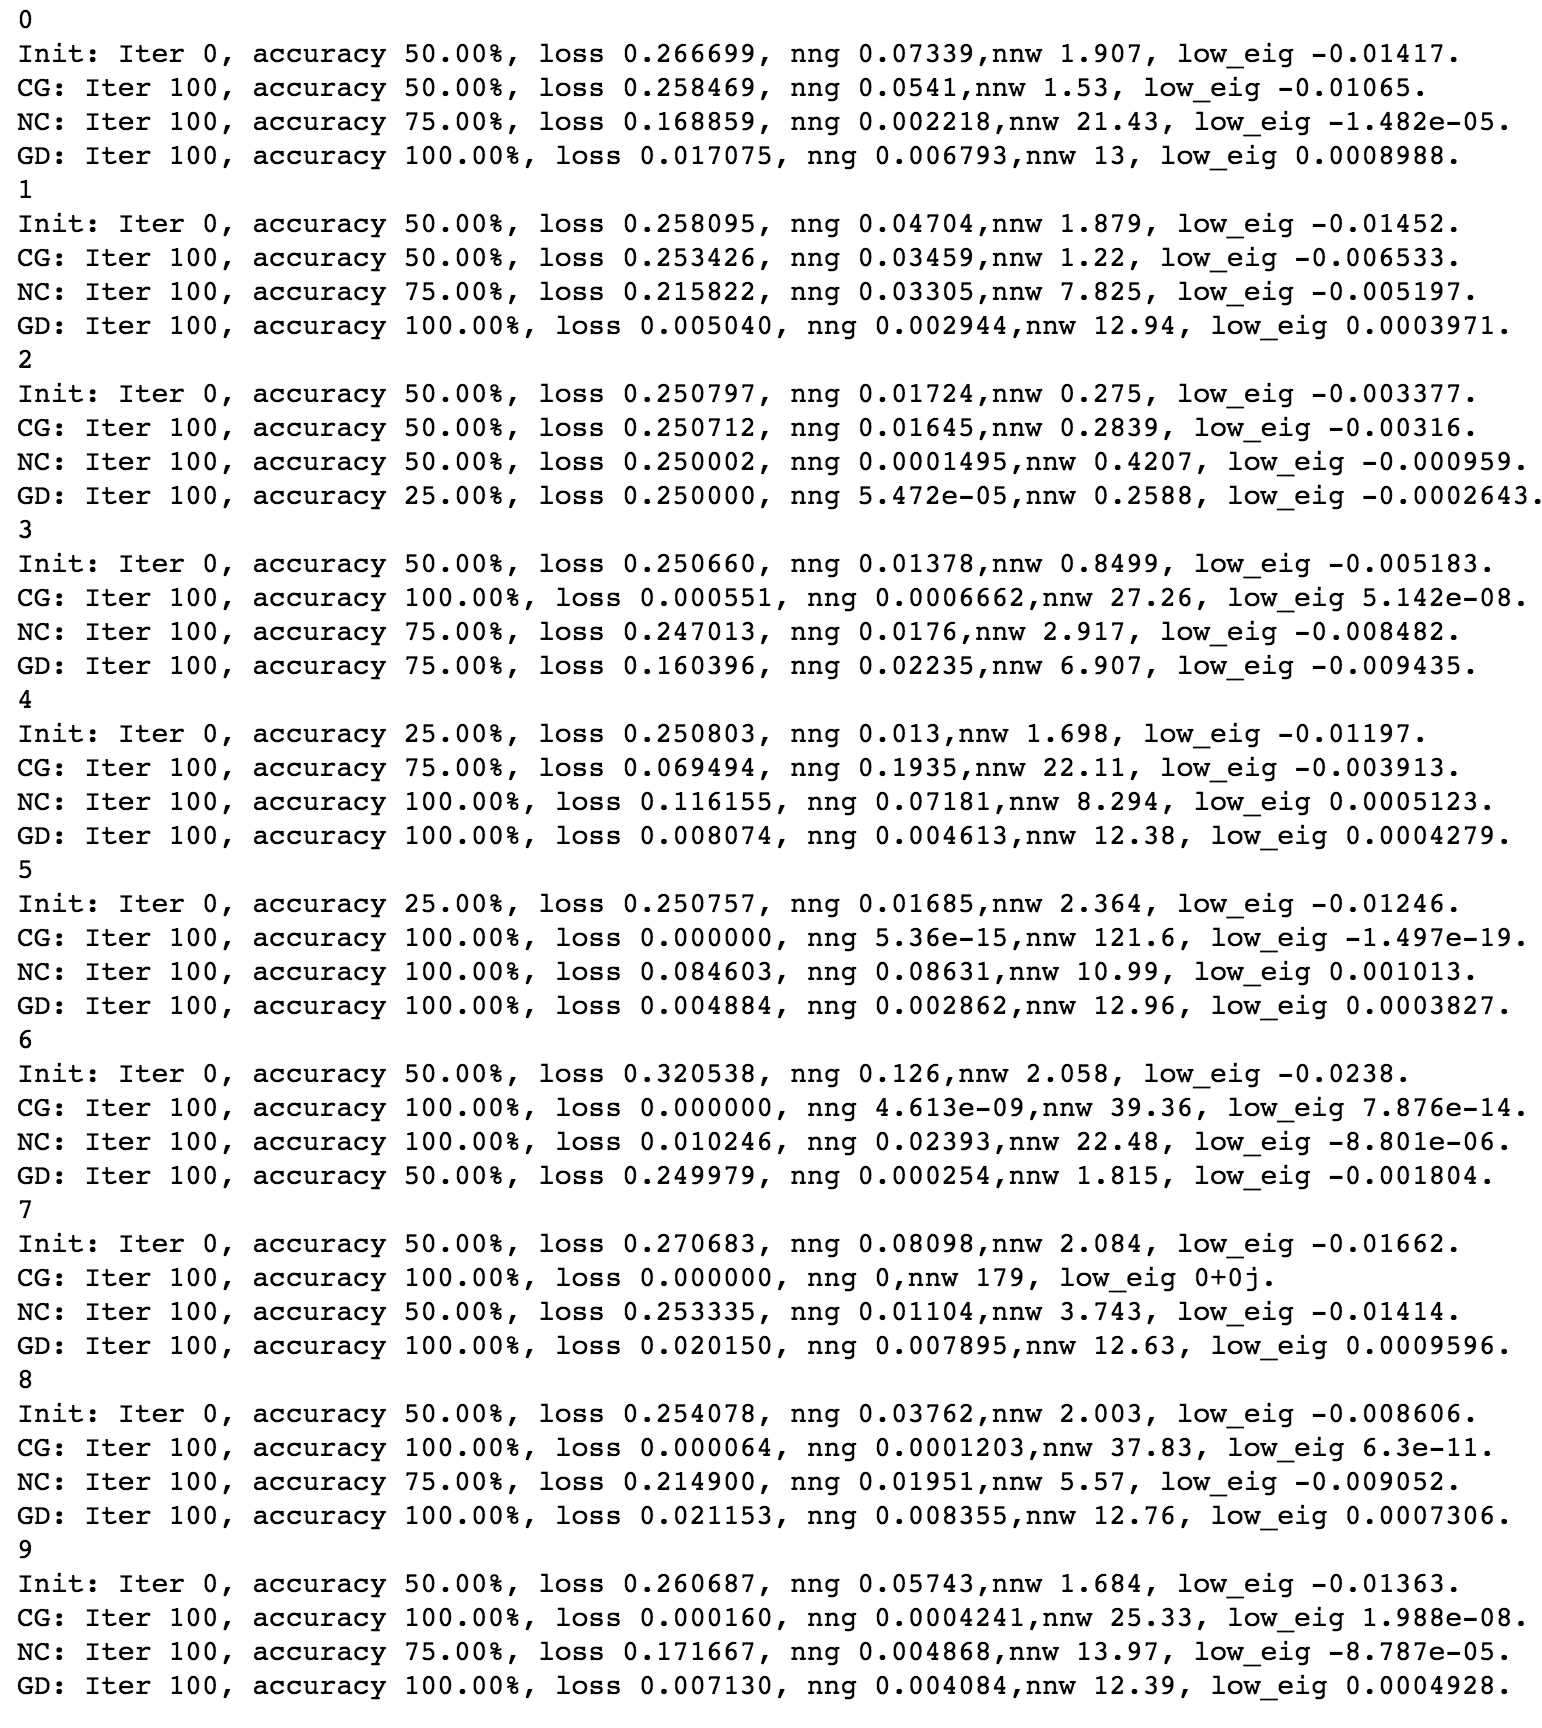
\includegraphics[width=16cm]{threeM}
\caption{}
\label{fig:3m}
\end{figure}



\section{Visualization of these directions on N2}

In all the experiments, we only use N1 as the network structure. Here we consider to use N2 to build visualization which help to understand different kinds of directions. Note that we will fix the value of two biases so that there will be only 2 weights as parameters. Figure~\ref{fig:landscape} shows an example of such visualization. The axis having the range from $0.25$ to $0.5$ represents the objective value, while the other two represent the values of two weights. The black, red and blue lines represents leftmost eigenvector, CG outputs and negative gradient directions respectively. I hope visualization like this will be helpful in future exploration.  

\begin{figure}[t]
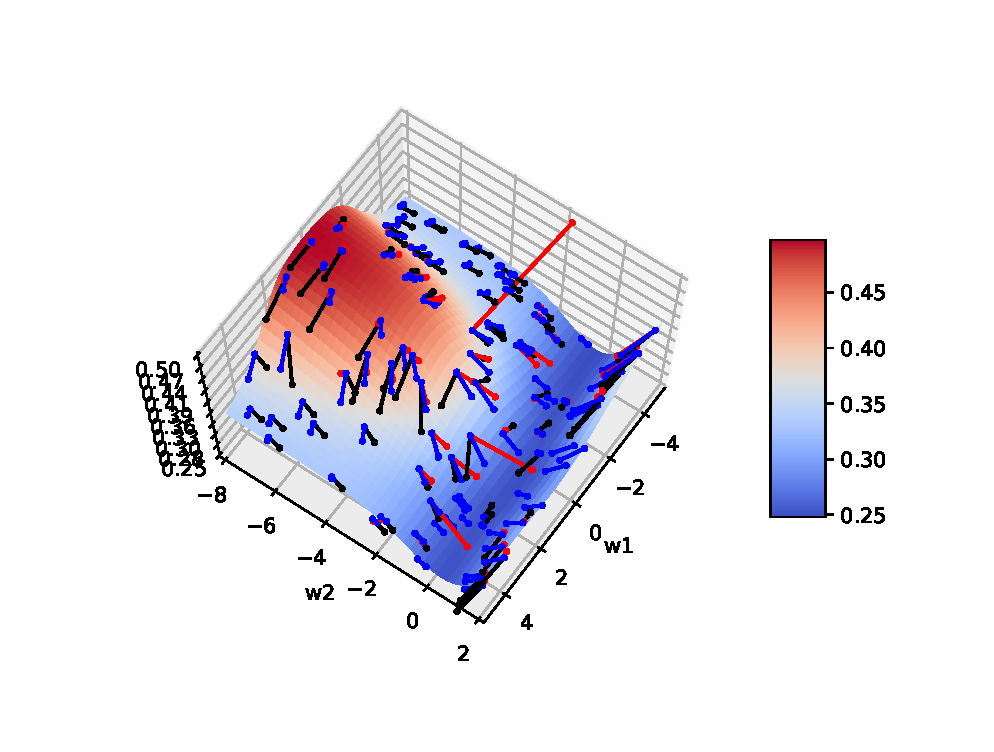
\includegraphics[width=15cm]{2w.eps}
\caption{Landscape of network N2 by fixing two biases and three kinds of directions at $100$ random points.}
\label{fig:landscape}
\end{figure}

\section{Next steps}
\begin{itemize}
\item Figure out the reason why CG performs better in Section 4 but worse in Section 2.
\item Improve current line search strategies.
\item Read the paper \cite{rr} and think about landscape of N1.
\end{itemize}

\begin{thebibliography}{9}
\bibitem{rr} 
Li, Hao, Zheng Xu, Gavin Taylor, and Tom Goldstein. 
"Visualizing the Loss Landscap of Neural Nets." arXiv preprint arXiv:1712.09913 (2017). 
\end{thebibliography}

\end{document}	



